\section{Calibration} \label{sec:calib}

In this section the various calibration procedures taken in order to minimize the time resolution and enhance both the particle identification (PID) and time of flight (TOF) capabilities of the Start Counter are discussed.

\subsection{Time-walk Correction} \label{sec:calib_tw}

The time-walk effect is a well understood consequence of leading edge discriminators (LED).  Analog signals of varying amplitudes crossing a fixed threshold, as determined by the discriminator threshold setting, will do so at varying times. %as illustrated in Fig.~\ref{fig:time_walk_effect}.
%	\begin{figure}[!htb]
%		\centering
%		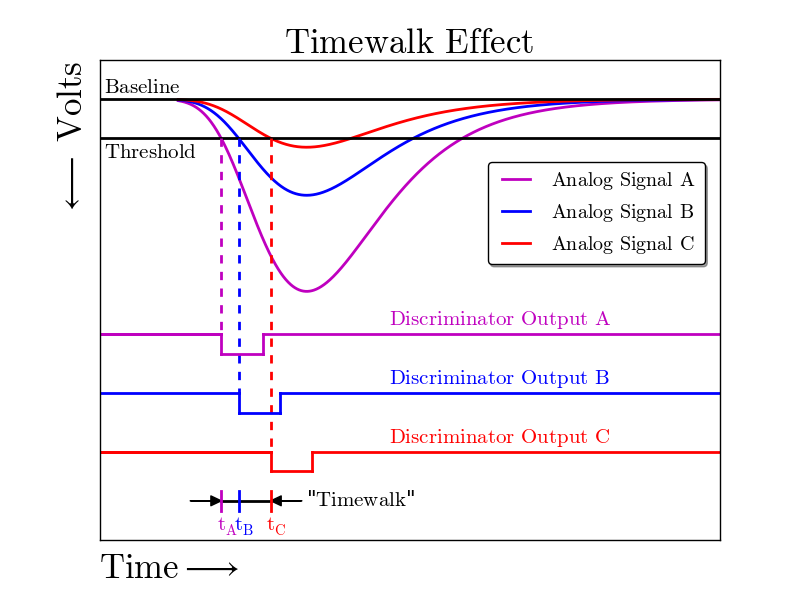
\includegraphics[width=1.0\columnwidth]{calibration/figs/time_walk_effect}
%		\caption{Example of the time-walk effect. Three coincident analog signals A, B, \& C of varying amplitudes crossing a fixed threshold in a LED. The discriminator logic output signals vary in time relative to the amplitude of the incoming analog signal.  The signals shown above are simulated analog signals being fed into the LED's thus, they have negative polarity.}
%		\label{fig:time_walk_effect}
%	\end{figure}
Thus, the corresponding logic signal output from the LED will ``\textit{walk about}'' in time, resulting in an undesirable smearing of the measured ST TDC times.

The FADC250's provide a high resolution pulse time (62.5~ps) that is time-walk independent \cite{pooser16} \cite{dong_fadc}.  
% WB here the question will come why bother with a discriminator then ?  
% EP I would argue the the mutihit capability (> number of FADC hits) and better resolution of the TDC's justify it's existance
Therefore, for events in which both the FADC and TDC register hits in the same channel, the pulse time can serve as a reference time for that event.  The TDC/FADC time difference is given by Eq.~\ref{eq:tdc_adc_tdiff}.
	\begin{equation} \label{eq:tdc_adc_tdiff}
		\delta t_{i} = t^{TDC}_{i} - t^{FADC}_{i}
	\end{equation}
Figure \ref{fig:twdistuncorrch15} shows a typical time-walk spectrum, \textit{i.e.} $\delta t_{i}$ versus the pulse amplitude, for one sector of the ST.
	\begin{figure}[!htb]
		\centering
		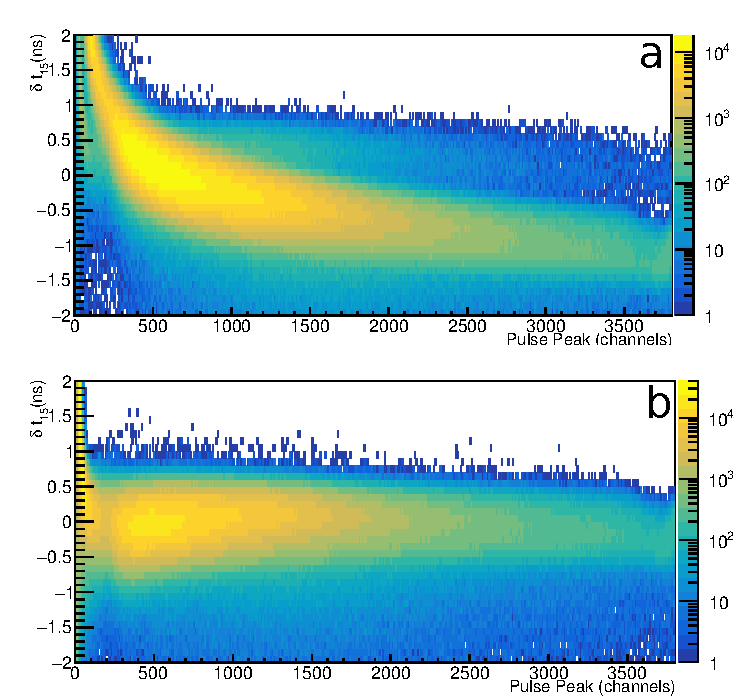
\includegraphics[width=1.07\columnwidth]{calibration/figs/NIM_TW.pdf}
		\caption{a) Typical Start Counter time-walk spectrum.  Shown is the time-walk spectrum for sector 15 of the Start Counter during the Spring 2017 run. On the y-axis is $\delta t_{15}$ and on the x-axis is the corresponding pedestal subtracted pulse peak spectrum. b) Same spectrum after walk correction.}
		\label{fig:twdistuncorrch15}
	\end{figure}
The FADC250's return both the amplitude and integral of events which are above threshold \cite{dong_fadc}.  Since the amplitude better characterizes the rise time of the ADC pulse profile as compared to the pulse integral, it was selected for the time-walk corrections.

Fig.~\ref{fig:twdistuncorrch15}-a shows the correlation between $\delta t{i}$ and the pedestal subtracted pulse amplitude for hits in sector 15 of the ST.  This correlation is nonlinear and requires a polynomial functional form to describe it. Equation~\ref{eq:tw_corr_func_form} from Ref.~\cite{esmith_bcal} was chosen to characterize the correlation between $\delta t_{i}$ and the amplitude of the signal. 
	\begin{equation} \label{eq:tw_corr_func_form}
		f^{w}_{i}\left(a/a^{thresh}_{i}\right) = c0_{i} + \frac{c1_{i}}{(a/a^{thresh}_{i})^{c2_{i}}}
	\end{equation}

In Eq.~\ref{eq:tw_corr_func_form} $f^{w}_{i}$ is the functional form of time-walk fit for the $i^{th}$ sector, while $a$ and $a^{thresh}_{i}$ are the pulse amplitude and discriminator threshold converted to ADC units respectively.  Furthermore, $c0_{i}, c1_{i}, c2_{i}$ are the time-walk correction fit parameters.  This empirical function was chosen so that as the pulse amplitude increases, the correction function will asymptotically approach a constant, namely $c0_{i}$.  Therefore, at large pulse amplitudes the correction $f^{w}_{i}$ for $\delta t_{i}$ will reduce to an effective offset.  Moreover, signals with small amplitudes will have $\delta t_{i}$, corrected \textit{via.} $f^{w}_{i}$, so as to match the signals with large amplitudes.  Thus, signals of varying amplitude will exhibit a constant $\delta t_{i}$ as desired.
% WB what is the relation between \delta t_i  and f here. I think this would be useful 
% EP done.

The data in Fig.~\ref{fig:twdistuncorrch15} were fit using Eq.~\ref{eq:tw_corr_func_form} and ROOT's MINUIT $\chi^{2}$ minimization fitting library \cite{root_minuit} for pulse peak values ranging from [50, 2100].  An identical fit was carried out for each of the ST sectors. 

% WB I would show the fitted function as illustration on the same graph
% EP Agreed, I was am on MK to provide the plots/fits

The most probable value (MPV) of the minimum ionizing peak was chosen to be the location in which the time-walk correction was zero.  This location effectively serves as a reference point for the correction.  
% WB I would skip this
% EP done
%As seen in Fig. \ref{fig:pulsepeakch15} a ``pseudo'' MPV was utilized.
%	\begin{figure}[!htb]
%		\centering
%		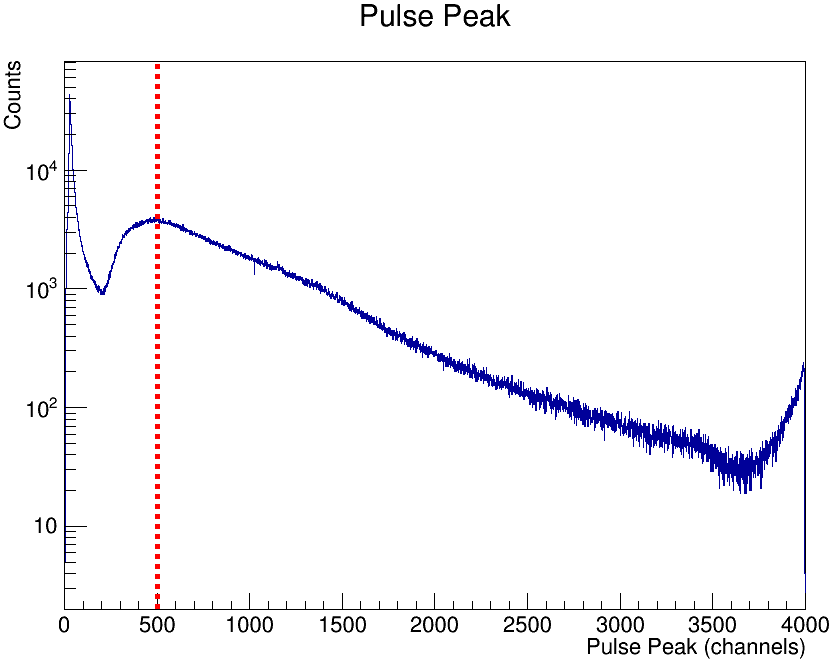
\includegraphics[width=1.0\columnwidth]{calibration/figs/pulse_peak_ch15}
%		\caption{Typical pulse peak minimum ionizing distribution.  Shown is the pulse peak minimum ionizing distribution for sector 3 during the Spring 2017 run. The red, vertical, dashed line in the histogram corresponds to the ``pseudo'' MPV ($a^{0}_{15}$) which was determined to be 500.}
%		\label{fig:pulsepeakch15}
%	\end{figure}
The MPV $(a^{0}_{i})$ was determined on a sector by sector basis by simply acquiring the pulse peak channel which had the most number of entries after the pulse peak channel 200.  The large spike in the pulse peak spectrum at very low pulse peak values are due to electromagnetic background events clipping threshold and do not correspond to a true minimum ionizing particle traversing the scintillator medium.

Once the necessary time-walk correction parameters are determined, the correction is applied to the TDC time and is illustrated by Eq. \ref{eq:tw_corr}.
	\begin{equation} \label{eq:tw_corr}
		T^{w}_{i} = t^{TDC}_{i} - f^{w}_{i}(a/a^{thresh}_{i}) + f^{w}_{i}(a^{0}_{i}/a^{thresh}_{i})
	\end{equation}
With the time walk corrections having been applied, the corrected timing distributions appear much more uniform in nature and exhibit a factor 1.75 improvement in resolution \cite{pooser16}.  Fig.~\ref{fig:twdistuncorrch15}-b illustrates the vast improvement in the time difference spectrum ($\delta t_{15}$) due to the applied time-walk corrections.
%	\begin{figure}[!htb]
%		\centering
%		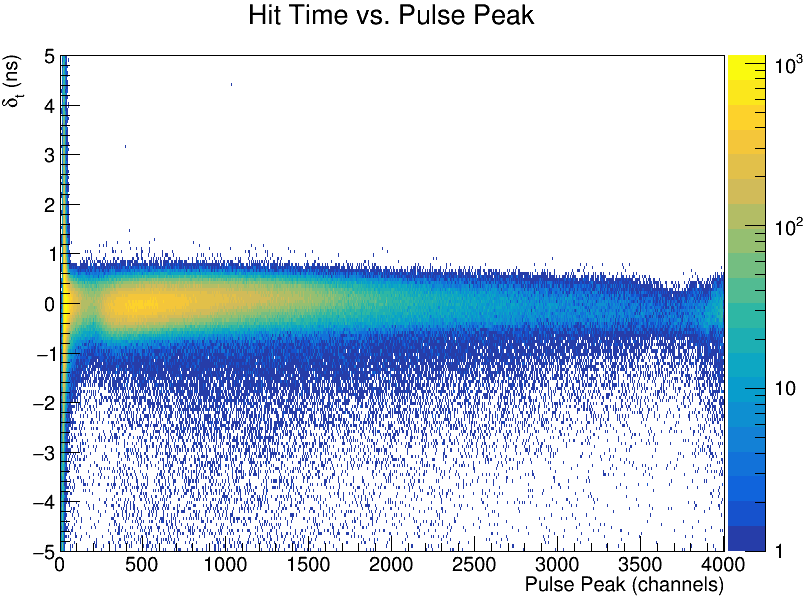
\includegraphics[width=1.0\columnwidth]{calibration/figs/tw_dist_corr_ch15}
%		\caption{Time-walk corrected time difference spectrum.  Shown is the time-walk %corrected time difference spectrum for sector 3 during the Spring 2017 run. The time-walk %corrected time difference spectrum has $\sigma_{\delta t_{15}} \approx 270 ps$}
%		\label{fig:twdistcorrch15}
%	\end{figure}
%Figure~\ref{fig:sttimeoverlaych15} illustrates the $\delta t_{15}$ distribution and the %relative effects of the aforementioned time-walk correction.
%	\begin{figure}[!htb]
%		\centering
%		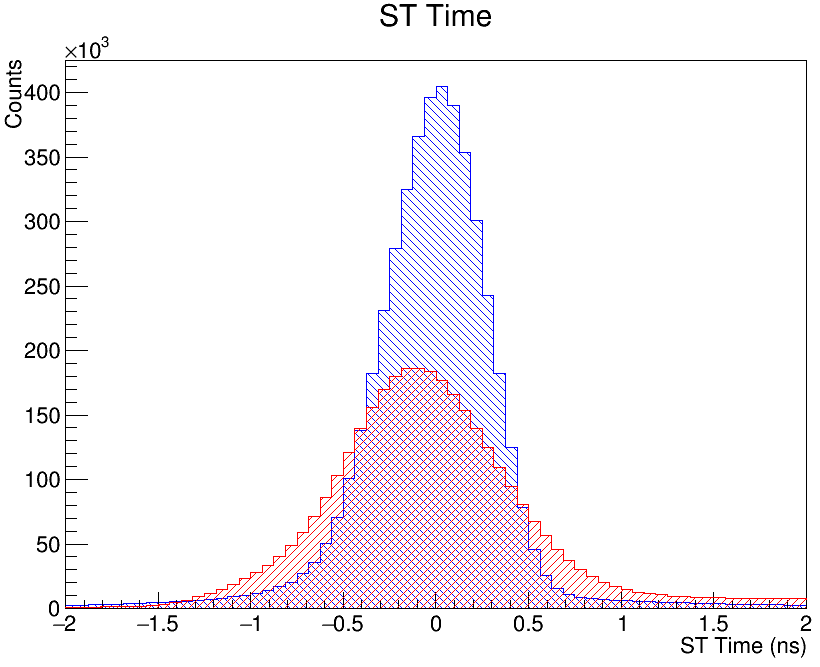
\includegraphics[width=1.0\columnwidth]{calibration/figs/st_time_overlay_ch15}
%		\caption{Comparison of pre and post self-timing distributions.}
%		\label{fig:sttimeoverlaych15}
%	\end{figure}

\subsection{Propagation Time Corrections} \label{sec:calib_ptc}

As a charged particle traverses through the ST scintillator material the molecules become excited and a small fraction $(\approx 3\%)$ \cite{pdg_2012} of the excitation energy is released in the form of ``optical'' photons.  The photons produced will be emitted uniformly in all directions and some will escape the medium, some will be reflected back into the medium by virtue of the reflective Al foil wrapping, and some will be lost.  However, the majority of detected  photons will have undergone many total internal reflections while they propagated from their source to the SiPM detector placed at the upstream end.  The time between production in the ST scintillator paddles and detection is position dependent and must be accounted for and is discussed below.

The EJ-200 scintillator material has a refractive index of 1.58 \cite{ej200_specs} and the corresponding speed of light is $\approx \mathrm{19\ cm/ns}$.  However, what is measured in the lab is known as the effective velocity which is slower due to the fact that the majority of photons are not traveling in straight lines parallel to the medium boundaries.  Instead they are constantly reflecting off the boundaries resulting in increased respective path lengths which contributes to a reduced velocity known as the effective velocity.  

Correcting for the time in which light spends traversing through the scintillator material is a necessary correction since the ST paddles are 60~cm in length.  Thus, light produced in the tip of the nose will take on the order of 4~ns to reach the SiPM at the upstream end.  Performing the propagation time corrections utilizing the common effective velocity method is not the most robust procedure for the case of the ST.  Studies performed with simulation and data showed that the unique geometry in the nose causes the effective velocity of light to be larger than that of the straight section and therefore they must be treated in an independent manner.

In order to conduct the propagation time corrections for the ST a distinct set of events needed to be selected so that a well defined reference time was being utilized.  This reference time was utilized as a measure of the event time for all other charged tracks intersecting the ST within the same event.  

For every charged track in a given event, two global tracking requirements were required.  First, only charged tracks with a good tracking confidence level were considered.  Secondly all charged tracks were required to have their vertex located within the target and radially within 1 cm from the beam. Only tracks passing these conditions were considered for analysis.

Two specific tracks were required in each event in order to conduct the ST propagation time corrections.  One track that has hit the time of flight (TOF) detector and not the ST provides the reference time for that event.  A separate track that has hit the ST and not the TOF was used to provide the ST measure of the vertex time.  This was done in order to avoid any potential bias in the calibration.  
	
% WB this is too detailed and technical. Refer to thesis and summarize the essential. From here to ...	
% EP done.

The advantage of using the time associated with a track matched to the TOF is that the time resolution of the TOF is the best of any detector in Hall-D $(\approx 96\ \mathrm{ps})$ \cite{zihlmann_tof}. The calibrated (time-walk \& propagation) hit time returned by the TOF $(T^{TOF}_{hit})$ was then corrected for the flight time from the track vertex to the TOF $(T^{TOF}_{flight})$.  Equation~\ref{eq:tof_vertex_time} is the TOF measure of the track vertex time.
	\begin{equation} \label{eq:tof_vertex_time}
		T^{TOF}_{vertex} = T^{TOF}_{hit} - T^{TOF}_{flight}
	\end{equation}

In order to determine the time in which the beam bunch arrived at the interaction point ($T^{BB}_{vertex}$) the $T^{TOF}_{vertex}$ time must first be corrected for the RF measure of the vertex time ($T^{RF}_{vertex}$).  The steps required to correctly calculate $T^{BB}_{vertex}$ are discussed in detail in Ref.~\cite{pooser16}.  For every event, the first track satisfying the aforementioned fiducial track selection and is matched to the TOF will then have the associated $T^{BB}_{vertex}$ time calculated.  This time serves as the reference time for all other tracks that have intersected the ST in that event.

%The RF signal that is readout in Hall-D is provided by the CEBAF accelerator at a rate of 499 MHz (2.004 ns) while the beam bunches are produced at a rate of  249.5 MHz (4.008 ns).  The RF signal from the accelerator is multiplexed into TDC's however, the provided signal rate is too high to readout without causing overflow in the TDC buffers thus the RF signal is pre-scaled \cite{mattione_rf_wiki}.  The pre-scale factor was 128 and consequently the RF signal was readout every $\mathrm{128 \times 2.004\ ns = 256.512\ ns}$.  Thus, the time associated with the beam bucket that produced the event of interest must be calculated since it is not provided directly.

%For every event, the associated RF time is the pre-scaled time the RF signal arrived at the center of the target $(T^{RF}_{center})$. This time must be propagated out to the vertex location of the track since the photon responsible for the track spends a non-negligible finite amount of time traversing through the target before interacting with it. This propagation time $(T^{RF}_{prop})$ correction is given by Eq.~\ref{eq:rf_prop_time}
%	\begin{equation} \label{eq:rf_prop_time}
%		T^{RF}_{prop} = (z_{vertex} - z^{target}_{center}) \cdot \frac{1}{c} 
%	\end{equation} 
%Once the propagation time is summed with the centered RF time $(T^{RF}_{center})$ one obtains the measure of the RF time at the vertex of the track and is given by Eq. \ref{eq:rf_vertex_time}.
%\begin{equation} \label{eq:rf_vertex_time}
%	T^{RF}_{vertex} = T^{RF}_{center} + T^{RF}_{prop}
%\end{equation}

%Due to the inherent ambiguity associated with pre-scaling,  $T^{RF}_{vertex}$ is not the correct measurement of the time the beam bunch actually produced the track.  Therefore, one must ``step'' $T^{RF}_{vertex}$ to the time the track was produced as measured by $T^{TOF}_{vertex}$.  To do this one must first calculate the time difference $\delta T$ given by Eq. \ref{eq:rf_delta_t}.
%	\begin{equation} \label{eq:rf_delta_t}
%		\delta T = T^{TOF}_{vertex} - T^{RF}_{vertex}
%	\end{equation}
%Next, one must calculate the number of beam buckets $(N^{buckets}_{step})$ that have elapsed during the $\delta T$ time period and is given by Eq. \ref{eq:n_buckets_shift}, where $(N^{buckets}_{step})$ is rounded to the nearest integer.
%	\begin{equation} \label{eq:n_buckets_shift}
%		N^{buckets}_{step} = \frac{\delta T}{T^{BB}_{period}} = \frac{\delta T}{4.008\ ns}
%	\end{equation}
%Lastly one can now calculate the time the beam bunch arrived at the vertex that produced the track $(T^{BB}_{vertex})$ and is given by Eq. \ref{eq:bb_vertex_time}.
%	\begin{equation} \label{eq:bb_vertex_time}
%		T^{BB}_{vertex} = T^{RF}_{vertex} + T^{BB}_{period} \cdot N^{buckets}_{step}
%	\end{equation}

%For every event, the first track satisfying the aforementioned fiducial track selection and is matched to the TOF will then have the associated $T^{BB}_{vertex}$ time calculated.  This time serves as the reference time for all other tracks that have intersected the ST in that event.

% here

In order to properly calculate the propagation time ($T^{ST}_{prop}$) of photons produced by a charged track intersecting the ST, a few quantities must be known.  Particularly the time-walk corrected hit time ($T^{ST}_{hit}$), the flight time from the track vertex to the ST intersection point ($T^{ST}_{flight}$), and a well defined reference time corresponding to the event ($T^{BB}_{vertex}$).  With the reference time determined, all other charged tracks passing the previously discussed fiducial track selection and which have a match to the ST (and not the TOF) are analyzed.  Equation~\ref{eq:st_prop_time} illustrates the ST measure of the vertex time.
	\begin{equation} \label{eq:st_prop_time}
		T^{ST}_{prop} = T^{ST}_{hit} - T^{ST}_{flight} - T^{BB}_{vertex}
	\end{equation} 

This time difference is a direct measure of the amount of time the detected light produced by the intersecting charged track spent traversing the scintillator medium.  In order to perform the propagation time corrections the $z$-coordinate of the tracks intersection point with the ST was also recorded for every charged track intersecting the ST relative to the upstream end $(z^{ST}_{hit})$.  Once both $T^{ST}_{prop}$ and $z^{ST}_{hit}$ were calculated, the propagation correction calculation could be performed.  Figure~\ref{fig:proptimeuncorr}-a illustrates correlation between these two quantities.
	\begin{figure*}[!htb]
		\centering
		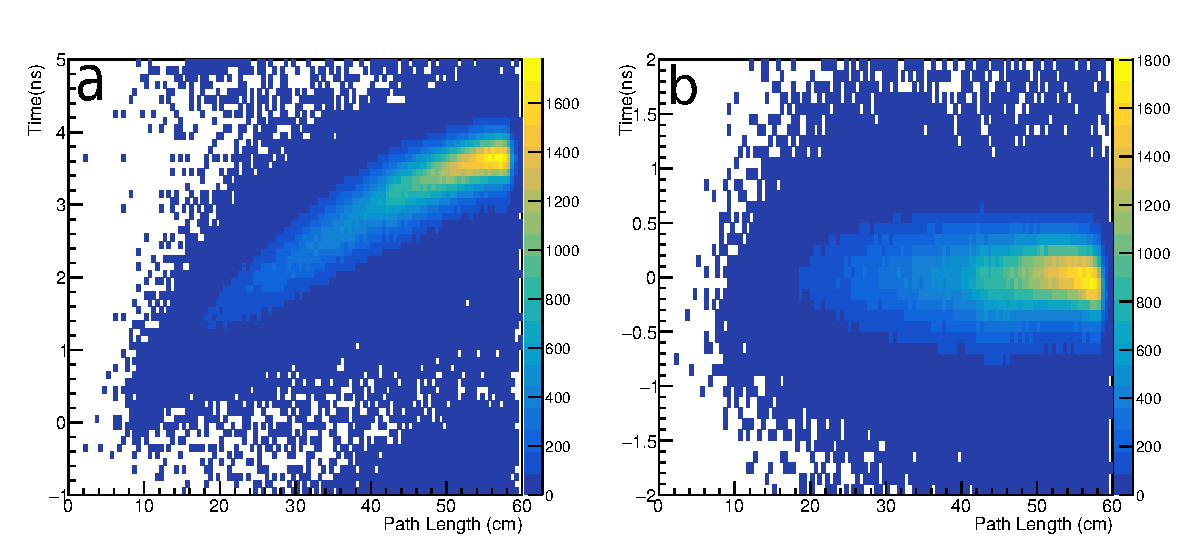
\includegraphics[width=1.0\textwidth]{calibration/figs/drawing}
		\caption{a) Typical Start Counter propagation time correlation.  Shown is the ST propagation time correlation for sector 15 of the ST during the Spring 2017 run 30279. $T^{ST}_{prop}$ is plotted on the y-axis and the $z^{ST}_{hit}$ is plotted along the x-axis, which represent the path length in cm. There is a clear correlation between the time in which optical photons are detected by the SiPM and the location of the charged track intersection point with the ST. b) Start Counter propagation time after correction}
		\label{fig:proptimeuncorr}
	\end{figure*}

The mean propagation times were then grouped into three distinct regions corresponding to the three unique geometrical sections of the ST namely the straight, bend, and nose regions.  These three regions were then fit utilizing the $\chi^{2}$ minimization technique with a linear function whose functional form is given by Eq. \ref{eq:pt_func_form} where the index $i$ indicates which region the fit is being performed.
	\begin{equation} \label{eq:pt_func_form}
		f_{i}(z) = A_{i} + B_{i} \cdot z
	\end{equation}
%The distributions and associated fits for the three regions are illustrated in %Fig.~\ref{fig:proptimeuncorrfits}.
%	\begin{figure}[!htb]
%		\centering
%		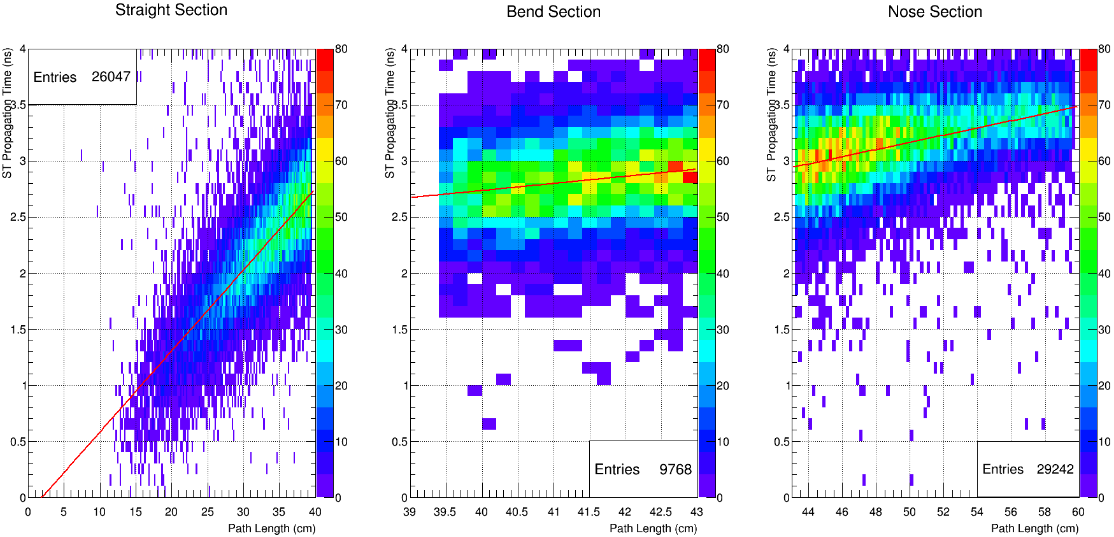
\includegraphics[width=1.0\columnwidth]{calibration/figs/prop_time_uncorr_fits}
%		\caption{Typical Start Counter propagation time projection correlation.  Left: Typical propagation time projection correlation for sector 15 of the ST during the Spring 2015 run 2931.  The red line serves as a reference for the propagation time assuming it was a constant 15 cm/ns.  The magenta line is the fit corresponding to the straight section.  The green and dark blue solid lines correspond to the fits in the bend and nose section respectively.  Right: zoomed in view of data points.}
%		\label{fig:proptimeuncorrfits}
%	\end{figure}
	
With the fit parameters determined an explicit time difference correction for each of the ST sectors could then be applied to calculate the ST measure of the vertex time given by Eq. \ref{eq:st_vertex_time}.
	\begin{equation}\label{eq:st_vertex_time}
	 	T^{ST}_{vertex}(z) = T^{ST}_{hit} - T^{ST}_{flight} - T^{ST}_{prop}(z)
	\end{equation} 
	
Figure ~\ref{fig:proptimeuncorr}-b illustrates the propagation time corrected ST time as a function of the path length of charged tracks match the the ST along the paddle up to the upstream end.
%\begin{figure}[!htb]
%	\centering
%	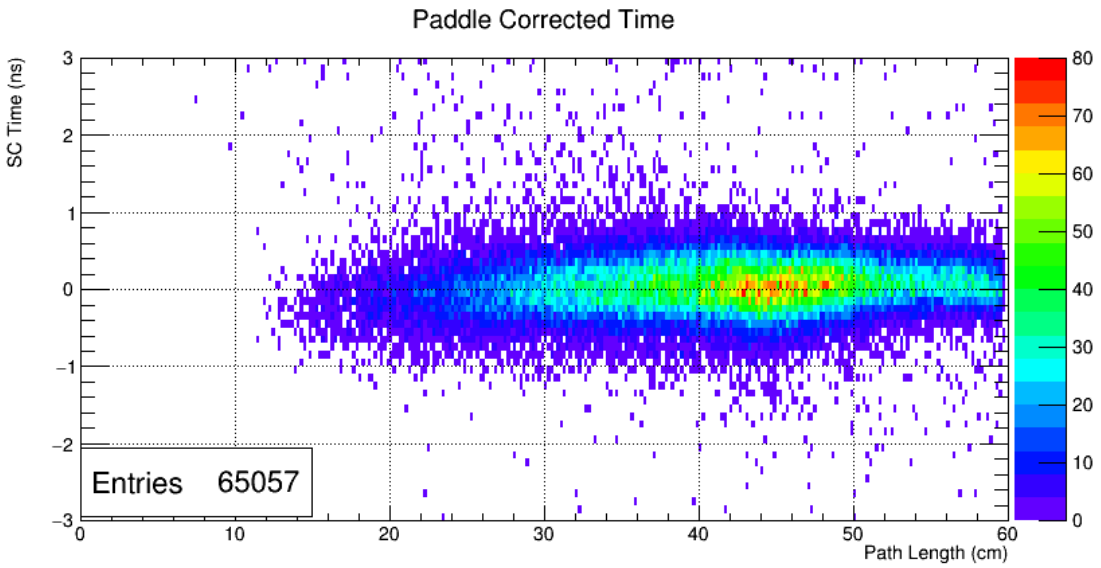
\includegraphics[width=1.0\columnwidth]{performance/figs/prop_time_corr}
%	\caption{Calibrated ST time versus the $z$-intersection of charged tracks matched to the %ST.}
%	\label{fig:proptimecorr}
%\end{figure}
In comparison to Fig.~\ref{fig:proptimeuncorr}-a, Fig.~\ref{fig:proptimeuncorr}-b no longer illustrates a dependence on the where the charged track intersects with the ST paddles as expected.
	
After the propagation time corrections are applied the ST corrected time now measures the vertex time for the track in the event and is discussed further in Sec.~\ref{sec:perform}

\subsection{Attenuation Corrections} \label{sec:calib_ac}

%Photons propagating in a scintillator medium can be lost through scattering, absorption, or escape at the boundaries.  

The measured energy deposited $(dE_{meas})$ from a charged particle traversing a scintillator medium is proportional to the number of photons created, which is in turn proportional to the integrated pulse read out by the FADC250. However, since the photons created \textit{via.} ionization can be lost through scattering, absorption, or escape at the boundaries as they propagate through the scintillator medium, the energy deposition measured by the SiPM does not correctly measure the energy deposited by the charged particle at the location of intersection with the scintillator and therefore must be corrected.  

% WB this was already described above
% EP agreed.
% Photons produced in a scintillator medium, as a result of charged particles traversing through the material,  are subject to the property of total internal reflection.  If the resulting photons incident on the scintillator-air boundary have an angle of incidence which is smaller than the critical angle, then the photons will leave the scintillator medium and be lost for detection and thus contribute to the overall attenuation.  However, if the incident  photon has an angle of incidence which is equal to or greater than the critical angle, $39.3^{\circ}$ for the ST scintillator-air interface \cite{pooser16}, then those photons will totally internally reflect and may possibly be detected.  The photons that do in fact totally internally reflect however, are still subject to additional phenomena which contribute to the overall attenuation of photons in the scintillator medium.  

One can define an \textit{attenuation coefficient} which characterizes a particular materials ability to absorb photons. The attenuation coefficient is defined to be the length in the medium in which the initial number of primary photons are reduced by a factor of $1/e$ (36.8\%).  Since the loss of photons in scintillators equates to the loss of information relative to the event of interest, it is desirable to have a scintillator material with a long attenuation length.  For reference a flat $2 \times 20 \times 300\ \mathrm{cm^{3}}$ EJ-200 scintillator has a relatively long attenuation length on the order of 4~m \cite{ej200_specs}.

In order to determine the attenuation coefficients of interest tracks hitting the ST, while passing identical fiducial track selection cuts as discussed in Sec.~\ref{sec:calib_ptc}, were selected for analysis.  Furthermore, the tracks pedestal subtracted pulse integral, energy deposition per unit length $(dE_{meas} / dx)$, and $z$-intersection with the ST relative to the upstream end, where the SiPM is located, were recorded.  

%A plot of the uncorrected energy deposition per unit length versus the track momentum $(dE_{meas} / dx\ vs.\ p)$ for tracks matched to the ST are shown in Fig.~\ref{fig:dEdx_vs_p_uncorr}.
	
%It is clear from Fig.~\ref{fig:dEdx_vs_p_uncorr}-a that no reliable PID can occur for tracks with $p > 0.6\ GeV/c$.
\begin{figure*}
		\centering
		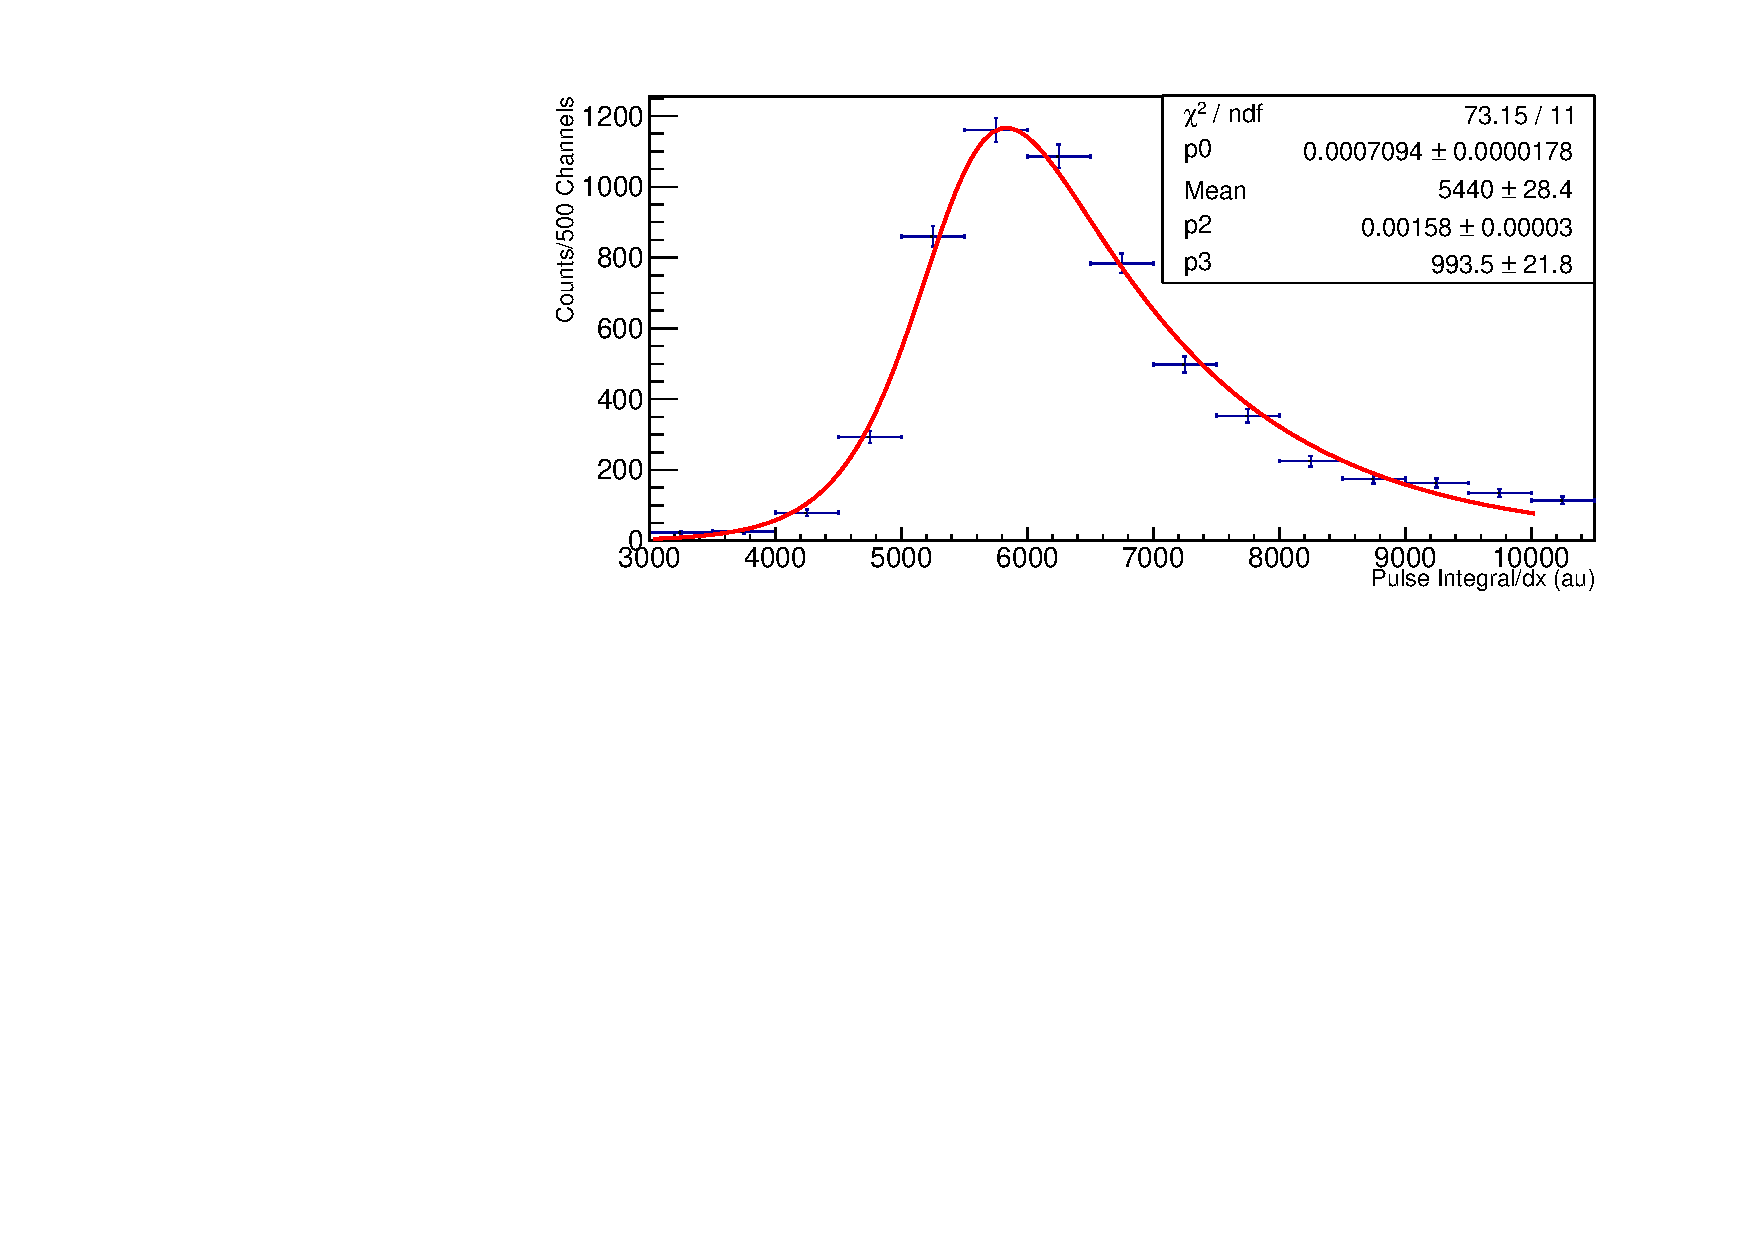
\includegraphics[width=1.05\textwidth]{calibration/figs/PiFit_sector15_int3}
		\caption{Empirical fits to extract the MPV of pedestal subtracted pulse integral FADC250 data in interval 3 along paddle 15.}
		\label{fig:pisecnosefits}
	\end{figure*}
The pedestal corrected pulse integral (PI), normalized to the path length $\mathrm{d}x$, data were binned in 3.5~cm $z$-intersection bins along the full length of the paddle. In order to properly quantify this data, the most probable value (MPV) of the data was extracted utilizing an empirical function given by equation \ref{mul:Fit Function}. 
%These data in the nose section are represented in Fig.~\ref{fig:pisecnose}.
% WB these variations can also come from different track angles, the pulse integrals should be corrected by dx
% EP agreed
%	\begin{figure}
%		\centering
%		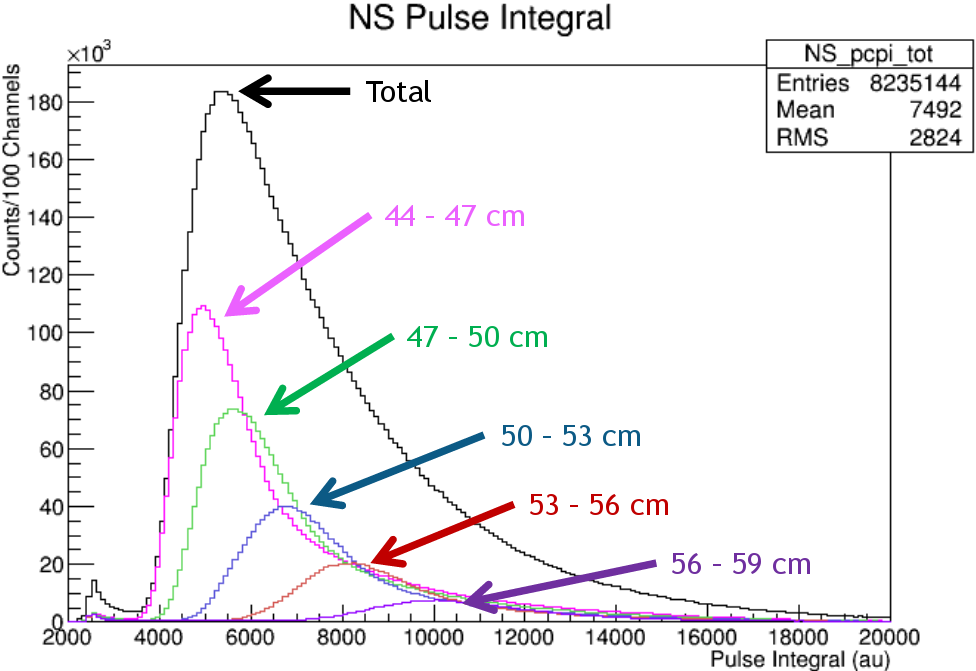
\includegraphics[width=1.0\columnwidth]{calibration/figs/pi_sec_nose}
%		\caption{Pedestal subtracted FADC pulse integral spectrum corresponding to the three ST sections.}
%		\label{fig:pisecnose}
%	\end{figure}


%	\begin{equation}\label{eq:Fit Function}
	\begin{multline}\label{mul:Fit Function}
	f(z)  = p_3 e^{(-p_0(z -Mean))} \\
	       \times (1+ \tanh(p_2(z-Mean))) 
	\end{multline}   
	
%In order to properly quantify this data, the most probable value (MPV) of the data was extracted utilizing the energy straggling distribution known as the Vavilov distribution \cite{vavilov_1957}.

%The Vavilov distribution, a generalization of the Landau distribution, is often utilized to describe the corresponding energy loss of charged particles traversing a thin layer of matter \cite{seltzer_1964}.  Unlike the more restrictive Landau distribution, the Vavilov distribution accounts for the maximum allowable energy transfer in a collision between a particle and an atomic electron \cite{schorr_1973}.  Therefore, the pulse integral data for each 1~cm bin along the the length of the ST paddles were fit utilizing the Vavilov distribution and the associated MPV was extracted.  
The fits to the data are illustrated in Fig.~\ref{fig:pisecnosefits}. 
	
With the MPV values extracted for each 3.5~cm $z$-intersection bin, the MPV values are plotted against the average $z$- value for each $z$-intersection bin as seen in Fig.~\ref{fig:attfits}.  This allows for one to quantitatively measure the attenuation of photons in the ST scintillators.


As was discussed in Sec.~\ref{sec:sim_mach} the unique geometry of the ST causes for mainly two distinct regions, \textit{i.e} straight and nose, to have differing properties in terms of light output and thus, time resolution.  Therefore, when performing attenuation corrections the two regions were treated independently in order to properly characterize photon attenuation.  
\begin{figure}[!htb]
	\centering
	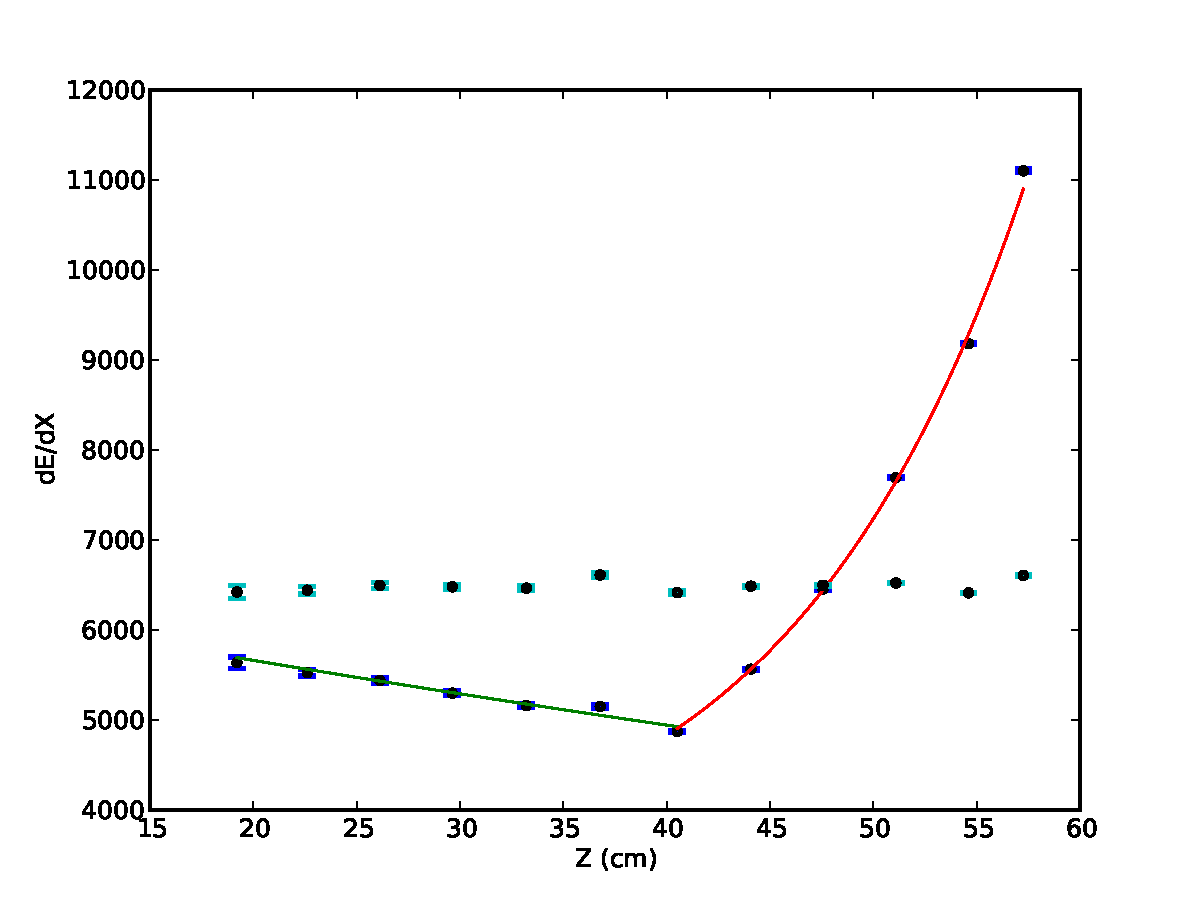
\includegraphics[width=1.06\columnwidth]{calibration/figs/Att_Fit15}
	\caption{Fits to the attenuation data.  The green line is the exponential fit from the upstream end up to the $Z_c$ while the red line is the exponential fit post $Z_c$ to the end of the nose section.  Results for sector 15 is shown before (blue error bars) and after corrections (cyan error bars).}
	\label{fig:attfits}
\end{figure}
It was empirically determined that the ideal fit function for the straight section would follow Eq. \ref{eq:ss_attn_ff_fit}.
	\begin{equation} \label{eq:ss_attn_ff_fit}
		f_{S}(z) = A_{S}e^{B_{S} \cdot z}
	\end{equation}
Similarly, the functional form of the nose section follows Eq. \ref{eq:bn_attn_ff_fit}.
	\begin{equation} \label{eq:bn_attn_ff_fit}
		f_{N}(z) = A_{N}e^{B_{N} \cdot z} + C_{N}
	\end{equation}
Exponential decay functions are typically used to describe the attenuations of photons in scintillator material.  However, for the unique case of the nose section, an exponential growth function was utilized. The boundary between applying the straight or the nose fit functions is determined by calculating the intersection point of the two fit functions $(Z_c)$. If ($z$) coordinate of the intersection point of the track is less than  $(Z_c)$, the straight correction is applied. Otherwise, the nose correction is used.

% WB I would skip the polynmial
% EP done.
Figure~\ref{fig:attfits} illustrates the pulse integral mean vs. average $z$-intersection along the paddle for sector 15.  

It is clear that the aforementioned exponential functions, corresponding to their respective geometrical sections, fit the data in a robust manner. 

Evaluating the fit function in the straight section at $z = 0\ \mathrm{cm}$ is representative of a minimum ionizing particle traversing through the upstream end closest to the SiPM readout.  In this instance the detected photons traverse through virtually no scintillator material, and are thus subject to no effects of attenuation.  Therefore, for all charged particles passing trough the ST scintillator paddles we apply an attenuation correction to the deposited energy measurement $(dE_{meas})$ to preserve the information regardless of where the track intersects the paddles.  
\begin{figure*}[!htb]
		\centering
		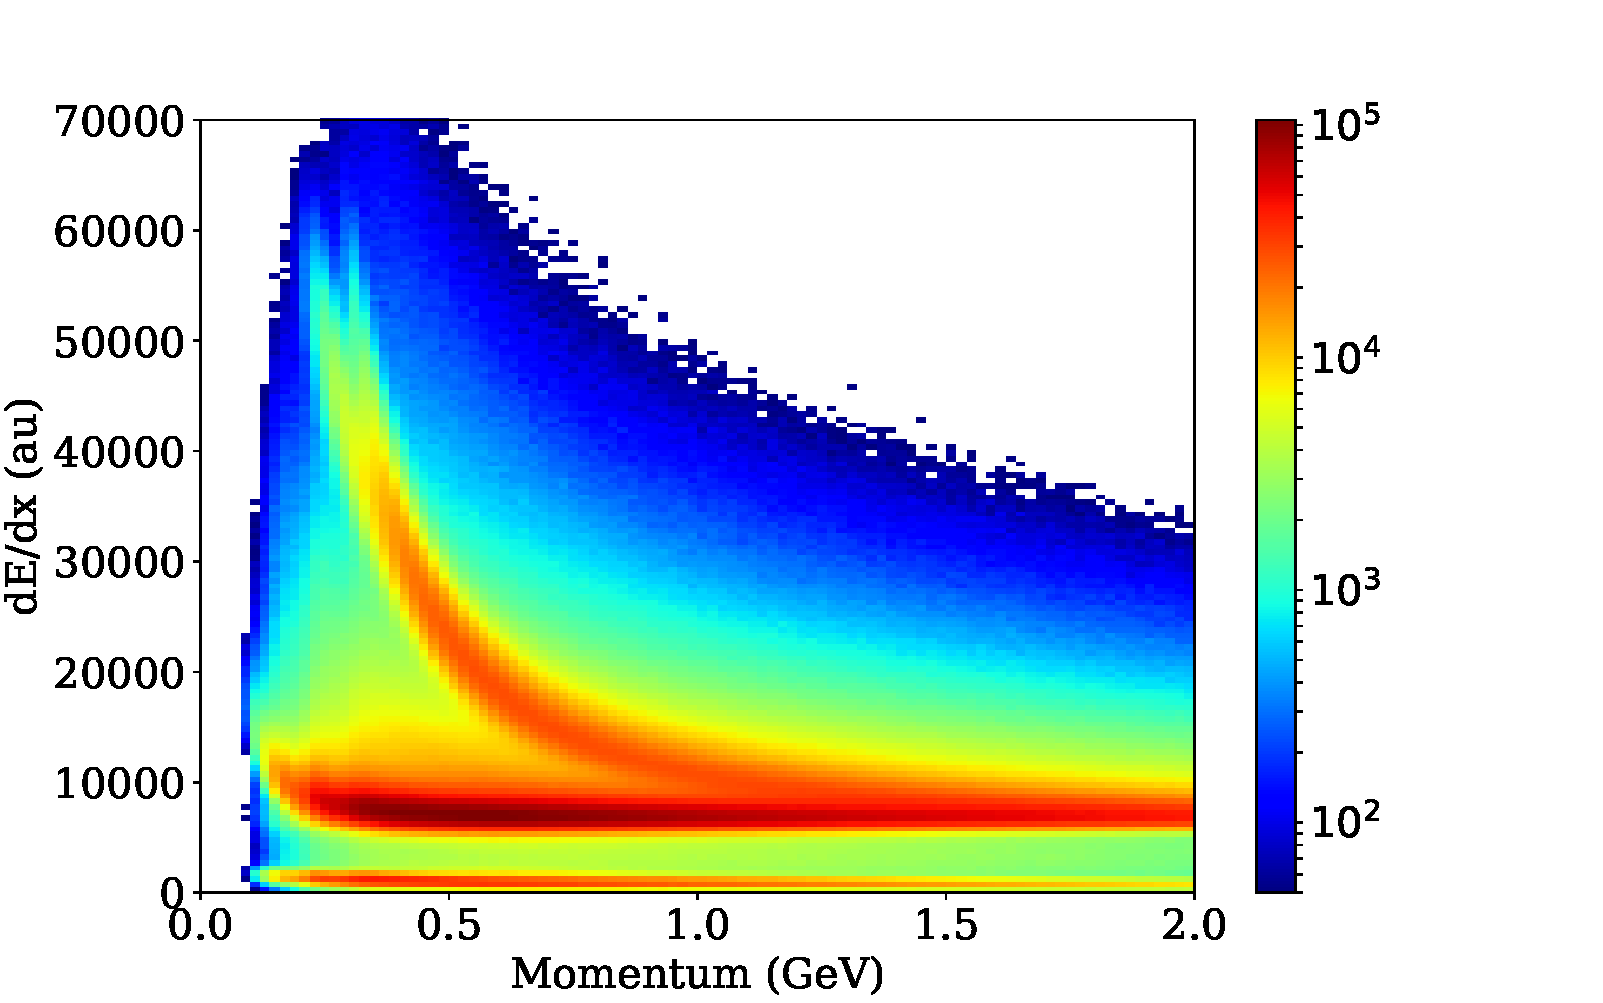
\includegraphics[width=1.0\textwidth]{calibration/figs/ATT_corr}
		\caption{Corrected $dE_{meas}/dx\ vs.\ p$ distribution in the Start Counter.  Shown is the distribution for tracks matched to the Start Counter in the Spring 2017 run 30279. The ``banana band'' corresponds to protons while the horizontal band corresponds to charged electrons, pions, and kaons.}
		\label{fig:dEdx_vs_p_uncorr}
	\end{figure*}
The gain of each paddle is not the same. Therefore a gain matching is performed using $f_{S}(0)$ of paddle 15 as a reference paddle. The gain matching factor is defined by equation 
 \ref{eq:GM}.
	\begin{equation} \label{eq:GM}
		GM = f_{S}(0)/f_{S}(0)_{Paddle 15}
	\end{equation}
	The corrected energy deposition $(dE_{corr})$ is given by Eq.~\ref{eq:gen_attn_corr} where the index $i$ indicates which section the charged track intersected with.
	\begin{equation} \label{eq:gen_attn_corr}
		dE_{corr} = dE_{meas} \cdot R_{i} /GM
	\end{equation}
For the straight section we have Eq.~\ref{eq:ss_attn_corr}.
	\begin{equation} \label{eq:ss_attn_corr}
		R_{S} = \frac{f_{S}(0.0)}{f_{S}(z)} = e^{-B_{S} \cdot z}
	\end{equation}
For the nose section we have Eq.~\ref{eq:bn_attn_corr}.
	\begin{equation} \label{eq:bn_attn_corr}
		R_{N} = \frac{f_{S}(0.0)}{f_{N}(z)} = \frac{A_{S}}{A_{N}e^{B_{N} \cdot z} + C_{N}}
	\end{equation}

Once all energy deposition measurements have had the appropriate attenuation corrections applied as was discussed above, the PID capabilities of the ST are considerably enhanced and are discussed further in Sec.~\ref{sec:perform}.
